%-------------------------------------------------------------------------------
% Document structure for report
%-------------------------------------------------------------------------------
\documentclass[a4paper]{article}
\usepackage[T1]{fontenc}
\usepackage[english]{babel} 
\usepackage{graphicx}
\usepackage{subcaption}
%\usepackage[utf8]{inputenc}
\graphicspath{ {images/} }
\usepackage[hidelinks]{hyperref}
\usepackage{multirow}
\usepackage{mathtools}

%-------------------------------------------------------------------------
% Start document with title page
%-------------------------------------------------------------------------
\begin{document}

\title{Laboratory Exercise \\Digital Visible and Infrared Imaging}
\author{
	Madeleine Bostr\"{o}m\\
	dat11mbo@student.lu.se
	\and
	Tobias Claesson\\
	ada10tcl@student.lu.se
}
\date{\today}
\maketitle

%-------------------------------------------------------------------------
% Actual document with sections
%-------------------------------------------------------------------------

\section{Introduction}
Digital images are stored as matrices containing data for what colour each pixel has. There are many different ways to analyze digital images, in this laboratory work we will see how to find the resolution of the image, experiment with different perspectives and how we can detect if something has changed in the image. We will also experiment using IR camera to detect what kind of material we can detect heat through.

\section{Theory}
\subsection{Magnification and resolution}
To measure the resolution we can use different methods such Rayleigh's criterion, modulation transfer function and point spread function. 
% A digital image has it's dimension in pixels and the resolution of digital images is the dimension of an image in pixels.
% The ratio between image and object size is known as the magnification for an optical system. 
% MTF Ratio between input and output modulation. 

\subsection{Grey scale images, image format and image information}
Every pixel stored in the matrix as unsigned integer, which means that we can encounter some problems when performing mathematical operations, eg 150+150=255 or 10-33=0. For this reason we temporarily convert the matrix using the formula I=double(I)/255. 

When subtracting two images one subtracts each pixel in the first matrix with the corresponding pixel in the other matrix. %http://homepages.inf.ed.ac.uk/rbf/HIPR2/pixsub.htm
This means that if we subtract to identical images we will only get a black image since the intensity in each pixel will be 0, this also means that we could detect movement in the picture since some pixels will be displaced in the second image and the result will no longer be 0.
\subsection{Histogram equalization}

\subsection{Colour images}

% Kom på något bättre till rubrik

\subsection{IR - Imaging}

\section{Method}
% Skriv en kort text innan subsectionerna 
\subsection{Pixel size, magnification and resolution}
To take images of an object we used a CCD camera and the m-file \texttt{takeImage.m} which gave us black and white images. In background of the object we had a test chart with horizontal and vertical lines with different distances between their lines. 

We used these images and MatLab functions such as \texttt{imcrop, size} and \texttt{getpts} to calculate how many pixels on the screen that corresponded to a centimeter, determined a distance in the image and also to compare vertical and horizontal resolution. 

\subsection{Grey scale images, image format and image information}
We started by loading the image and normalizing the intensity by dividing it by 255 and converting it to double. Then we used the \texttt{imcrop} command to select the part of the image we wanted to use. We then tested some different functions to show that we can show the image in different ways, such as the \texttt{flipud} command to flip the image upside down. 

After we got comfortable with the different commands and understood how we could manipulate the image we moved on to the next part of the assignment and made two new matrices from the image. The first matrix, lets call this I1, we removed the first row and in the second matrix, we will call this I2, we removed the last row. I1 now have shifted one pixel.
By using the test chart we determined the MTF-values by summing along the columns on a arbitrary row.

\subsection{Image enhancement}
We enhanced two images (see figure \ref{fig:img1org} and \ref{fig:img2org}) with histogram equalization and contrast stretching by using MatLab function \texttt{histeq} and \texttt{imhist}. 

\subsection{Colour images}
We took a colour photo using a camera and transferred it to the computer and examined the resolution. We then used the MatLab command \texttt{imhist} to compare the spectrum of different parts of the image. % Kanske ska se över denna meningen lite
We also studied a method that highlights every matching colour with the selected colour.

\subsection{IR - Imaging}
We used an infra-red camera to study heat conduction, friction heat and evaporation heat. We also studied the transmission, reflection, absorption and scattering properties of some objects such as water, glass, plastic and whiteboard.

\section{Results}
\subsection{Pixel size, magnification and resolution}
Our result from calculating how many pixels in the image (see figure \ref{fig:TestChart}) that corresponds to one centimetre were 41. When we calculated the length of a car in the image (see figure \ref{fig:Toy1}) we got the result 10 cm. When comparing the resolution from two images of a object at different distances, we got the result of more pixels per cm when closer to the object.

\begin{figure}[h]
	\centering
	\begin{subfigure}[b]{0.3\textwidth}
		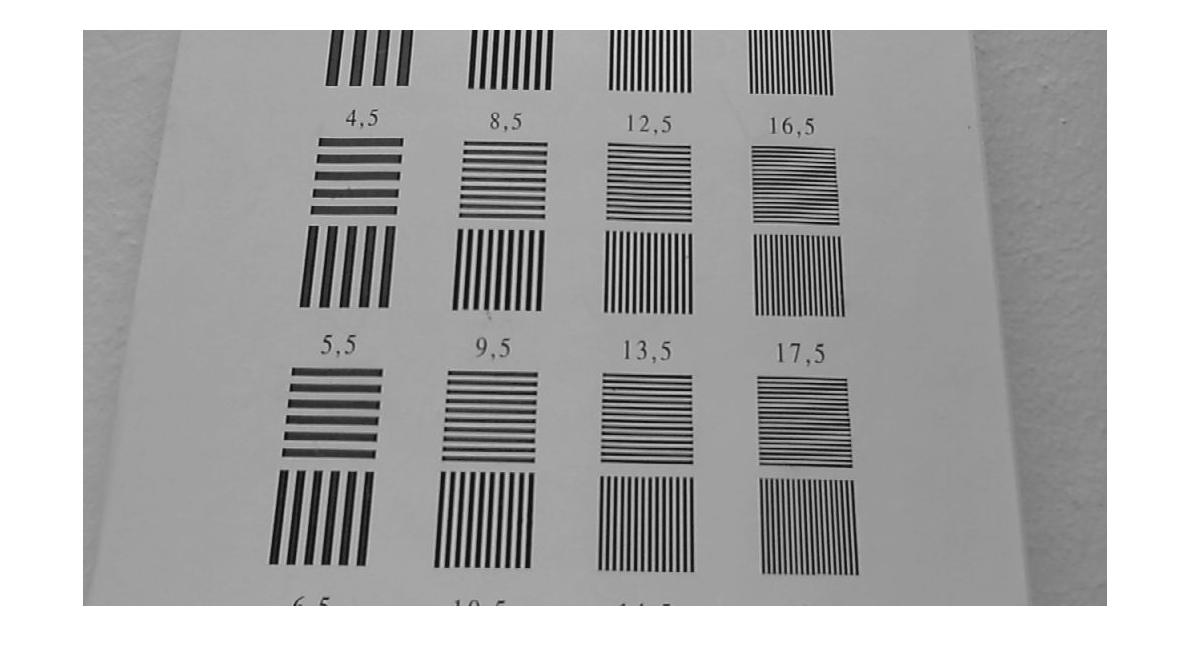
\includegraphics[width=\textwidth]{part1image1}
		\caption{}
		\label{fig:TestChart}
	\end{subfigure}
	\begin{subfigure}[b]{0.3\textwidth}
		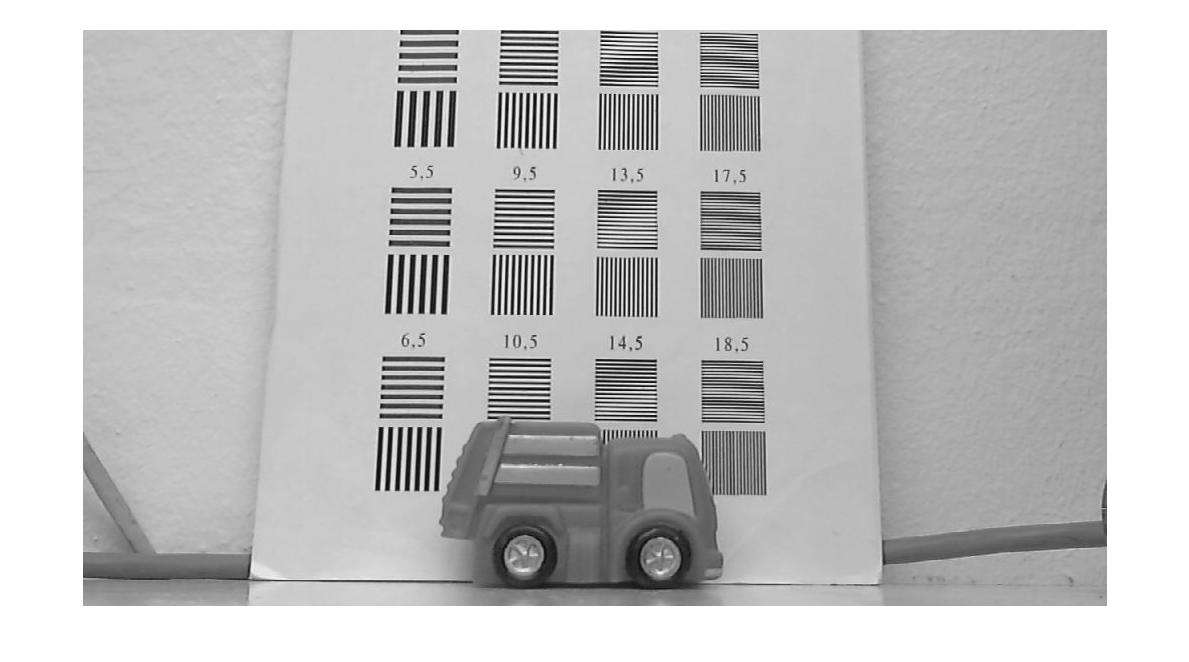
\includegraphics[width=\textwidth]{leksak1}
		\caption{}
		\label{fig:Toy1}
	\end{subfigure}
	\begin{subfigure}[b]{0.3\textwidth}
		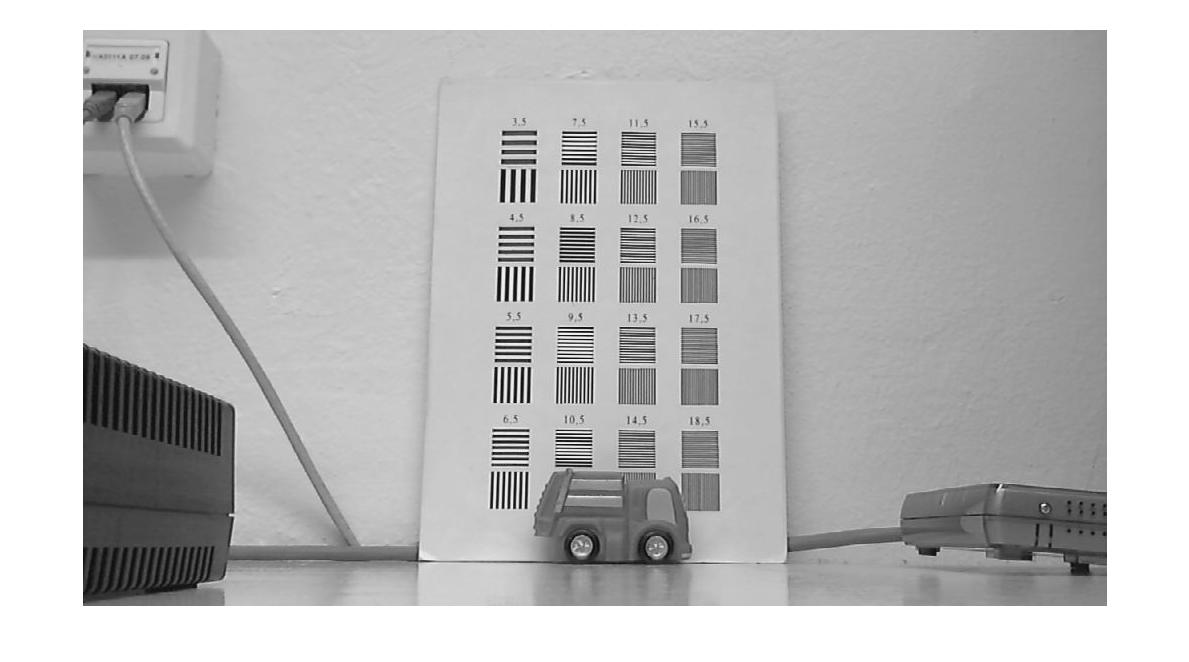
\includegraphics[width=\textwidth]{leksak2}
		\caption{}
		\label{fig:Toy2}
	\end{subfigure}
	\caption{(a) Image of test chart used to calculate how many pixels correspond to 1 cm. (b) Image used to measure distance of object and to compare the vertical and horizontal . (c) Image used to compare the resolution for different distances.}
	\label{fig:part1}
\end{figure}

\subsection{Grey scale images, image format and image information}
Our result from this part was A and B

\begin{figure}[h]
\centering
	\begin{subfigure}[b]{0.4\textwidth}
		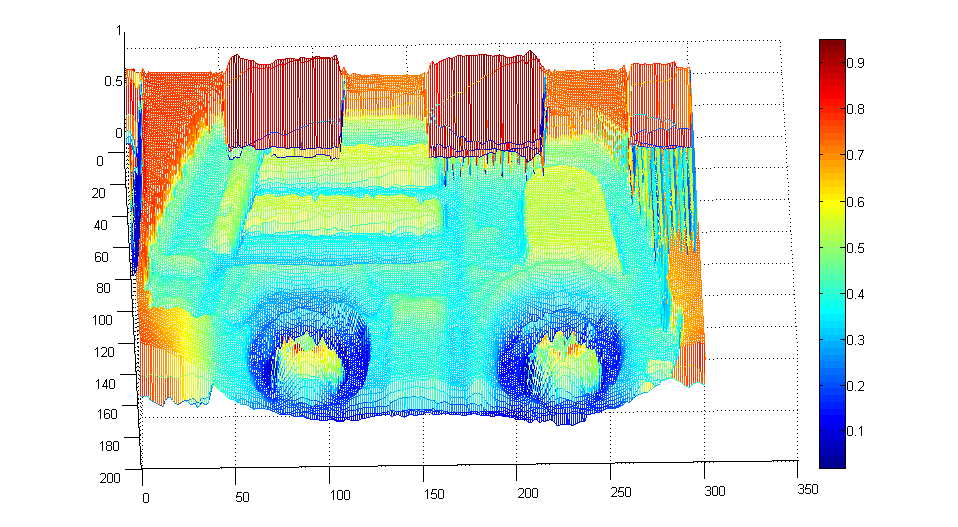
\includegraphics[width=\textwidth]{part2_mesh_croppedCar2}
		\caption{}
		\label{fig:meshCar}
	\end{subfigure}
	\begin{subfigure}[b]{0.4\textwidth}	
		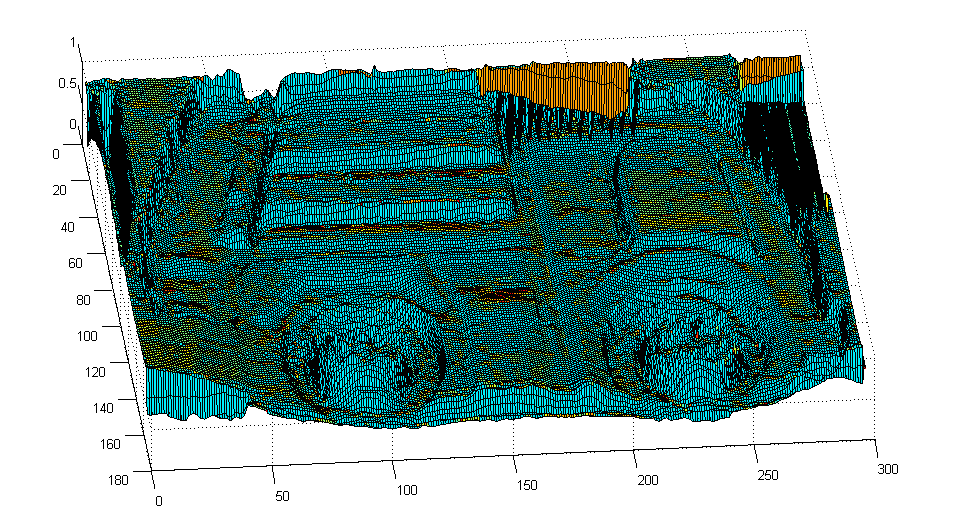
\includegraphics[width=\textwidth]{part2_surfl_croppedCar}
		\caption{}
		\label{fig:surflCar}
	\end{subfigure}
	\caption{(a) Matlab function mesh used on the cropped car image. (b) Matlab function surfl used on the cropped car image. }
	\label{fig:part2}
\end{figure}

\subsection{Image enhancement}
%\subsection{IR - Imaging}

\section{Discussion}
%discussion     ...we removed the last row because we wanted the matrices on the same format to be able to use subtraction. When we do the subtraction I1-I2 we will get the frames of the objects in the image. This is because of when we subtract each pixel with it's neighbor we will only se black if the two have the same color, and if the two pixels have different values, like the edge of the car and the background next to the car, we will see the frame of our object when the pixels are going from lighter to darker.


%grey values blabla function mesh shows different depths depending on what colour the pixels have

%-------------------------------------------------------------------------
% End of document - References follow
%-------------------------------------------------------------------------
\clearpage
\bibliographystyle{plain}
\begin{thebibliography}{count}
	\bibitem{introd-mtf}
	Introduction to Modulation Transfer Function. In Edmund optics. Retrieved November 22, 2014, from  http://www.edmundoptics.com/technical-resources-center/optics/modulation-transfer-function
	
	\bibitem{lab-hand}
	M. Brydegaard and S.G Pettersson,
	\emph{Laboratory Exercise Digital Visible and Infrared Imaging}, 2013
	
	\bibitem{mia-kth}
	Slides from Lecture 14, Medical Image Analysis, KTH. Retrieved November 22, 2014, from http://medim.sth.kth.se/6l2872/F/F9.pdf
	
	\bibitem{pix-sub}
	Pixel Subtraction. Retrieved November 22, 2014, from http://homepages.inf.ed.ac.uk/rbf/HIPR2/pixsub.htm
	
	\bibitem{enhanc-img}
	Shapiro and Stockman,
	\emph{Computer Vision, Chapter 5}, Mars 2000. Retrived November 22, 2014, from 
	https://courses.cs.washington.edu/courses/cse576/book/ch5.pdf
\end{thebibliography}

\end{document}